\documentclass[professionalfonts, aspectratio=169]{beamer}  
\usefonttheme{serif}                                        % Font theme: serif
\usepackage[utf8]{inputenc}                                 % Allows the use of different input encodings
\usepackage{graphicx}                                       % Enhanced support for graphics
\usepackage{amsmath}                                        % Enhances the typesetting of mathematics
\usepackage{amsfonts}                                       % Extra mathematical fonts
\usepackage{amssymb}                                        % Extra mathematical symbols
\usepackage{threeparttable}                 % For table notes
\usepackage{tikz}
\usetikzlibrary{shapes,arrows,positioning}
\usepackage{booktabs}                                       % Enhances the quality of tables
\usepackage{pgfplots}
\pgfplotsset{compat=1.17}
\usepackage{multirow}
% link settings
\usepackage{hyperref}                       % For hyperlinks
\usepackage[authoryear]{natbib}             % For bibliography

\usepackage{appendixnumberbeamer} % Numbering appendixes in beamer
\pdfstringdefDisableCommands{
  \def\translate{}
}
\usepackage{dcolumn}
\setbeamertemplate{navigation symbols}{} % Remove navigation symbols
\setbeamertemplate{footline}[frame number] % Add page number

% \setbeamercovered{transparent}  % Semi-transparent overlay

%---- Set the title page ----%
\title{Risk Adjustment, Self-Selection and Plan Design \\ in Medicare Advantage}
\institute{Stony Brook University}
\author{Zhu Liang}
\date{\today}

%---- Begin the document ----%
\begin{document}

\AtBeginSection[] % At the beginning of each section...
{
  \begin{frame}[noframenumbering, plain] % Create a new frame without a frame number
    \tableofcontents[currentsection] % Display the table of contents for the current section
  \end{frame}
}

\begin{frame}[noframenumbering, plain] % title frame without a frame number
    \titlepage
\end{frame}

%---- The slides structure ----%
\section{Introduction}

\begin{frame}{Managed Competition in Health Insurance}
  \begin{itemize}
    \item \textbf{Fee-for-Service (FFS)}:
      \begin{itemize}
        \item Government reimburses providers based on the actual services rendered to beneficiaries.
      \end{itemize}
    \item \textbf{Managed Competition}:
      \begin{itemize}
        \item Government provides fixed, predetermined subsidies (capitation) to insurance firms, independent of actual healthcare expenditures.
        \item Firms use these subsidies to offer insurance plans to beneficiaries.
      \end{itemize}
  \end{itemize}
\end{frame}    

\begin{frame}{An Example: Medicare Advantage}
% insert the picture from figures/images/medicare_market.tex and center it
\begin{figure}
  \centering
  \resizebox{0.6\textwidth}{!}{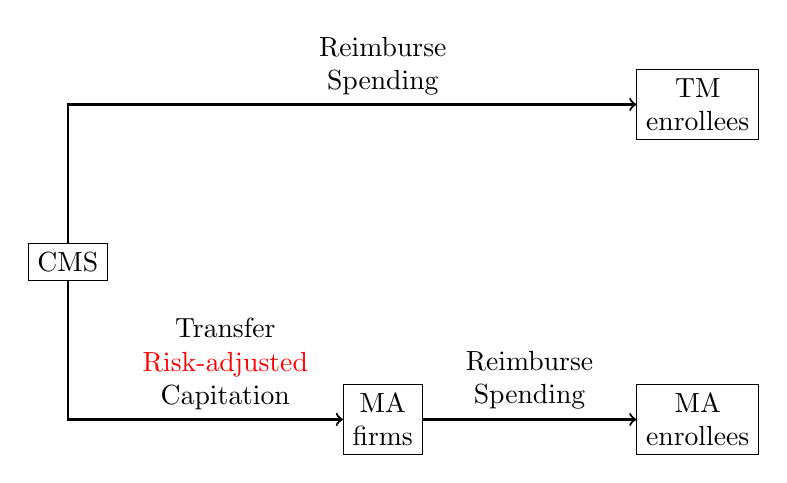
\begin{tikzpicture}
    \node[draw] (CMS) at (0,2) {CMS};
    \node[draw, align=center] (TM) at (8,4) {TM \\ enrollees};
    \node[draw, align=center] (MA) at (8,0) {MA \\ enrollees};
    \node[draw, align=center] (MAf) at (4,0) {MA \\ firms};

    \draw[->, thick] (CMS.north) |- (TM.west);
    \draw[->, thick] (CMS.south) |- (MAf.west);
    \draw[->, thick] (MAf.east) -- (MA.west) node[midway, above, align=center] {Reimburse \\ Spending};

    \node[above, align=center] at (4,4) {Reimburse \\ Spending};
    \node[above, align=center] at (2,0) {Transfer \\ \textcolor{red}{Risk-adjusted} \\ Capitation};
\end{tikzpicture}}
\end{figure}

\begin{itemize}\small
  \item Traditional Medicare (TM) is FFS.
  \item Medicare Advantage (MA) is managed competition.
  \item Beneficiaries choose between TM and MA.
\end{itemize}
\end{frame}

\begin{frame}{Selection in Health Insurance Markets}
  \begin{itemize}
    \item \textbf{Cream Skimming}: Insurance plans strategically target healthier beneficiaries to maximize profits
    \item \textbf{Risk Adjustment}: Government implements differential payments based on beneficiary risk profiles
    \item Can risk adjustment effectively neutralize insurers' incentives for cream skimming?
  \end{itemize}
\end{frame}

\begin{frame}{Simplified Risk Adjustment Scenario}
  \begin{itemize}
    \item Equal numbers of young and old individuals
    \begin{itemize}
      \item \textbf{Young}: 80\% healthy, 20\% sick
      \item \textbf{Old}: 20\% healthy, 80\% sick
    \end{itemize}
    \item Cost of care: \$1,000 for healthy individuals, \$5,000 for sick individuals
    \item Age is observable to gov; health status is not \pause
    \item Capitation risk-adjusted by age:
    \begin{itemize}
      \item \textbf{Young}: \$1,000 $\times$ 0.8 + \$5,000 $\times$ 0.2 = \$1,800
      \item \textbf{Old}: \$1,000 $\times$ 0.2 + \$5,000 $\times$ 0.8 = \$4,200
    \end{itemize}
    \item Average capitation rate based on health status:
    \begin{itemize}
      \item \textbf{Healthy}: \$1,800 $\times$ 0.8 + \$4,200 $\times$ 0.2 = \$2,040\ (\textbf{above} cost \$1,000)
      \item \textbf{Sick}: \$1,800 $\times$ 0.2 + \$4,200 $\times$ 0.8 = \$3,960\ (\textbf{below} cost \$5,000)
    \end{itemize}
    \item Firms still prefer \textbf{Healthy} individuals.
  \end{itemize}
\end{frame}

\begin{frame}{Self-Selection and Plan Design}
  \begin{itemize}
    \item When beneficiaries possess private information regarding their health status, they can engage in self-selection on plan choice.
    \item Firms can strategically design their plans to attract healthier individuals through this self-selection.
  \end{itemize}
\end{frame}

\begin{frame}{Research Question}
  \begin{itemize}
    \item How do interactions between plan design and self-selection influence the effectiveness of risk adjustment?
    \item What are the welfare implications arising from these interactions?
  \end{itemize}
\end{frame}

\begin{frame}{This Paper}
  \begin{itemize}
    \item Approach
    \item Results
  \end{itemize}
\end{frame}

\begin{frame}{Contributions}
  \begin{itemize}
    \item \textbf{Theoretical}: Develop a model of managed competition with endogenous plan design and self-selection with private information.
    \item \textbf{Empirical}: Estimate the model using data from Medicare Advantage.
    \item \textbf{Policy}: Evaluate the welfare implications of self-selection effect in health insurance markets.
  \end{itemize}
\end{frame}

\section{Data}
\section{Model}
\section{Results}

%---- The appendix ----%
\appendix
\begin{frame}[plain, noframenumbering] % Create a new frame without a frame number
  % show the title of the appendix centered on the slide
  \begin{center}
    \Huge Appendix
  \end{center}
\end{frame}

\begin{frame}{Appendix: Risk Adjustment Generation}
  \begin{figure}
    \centering
    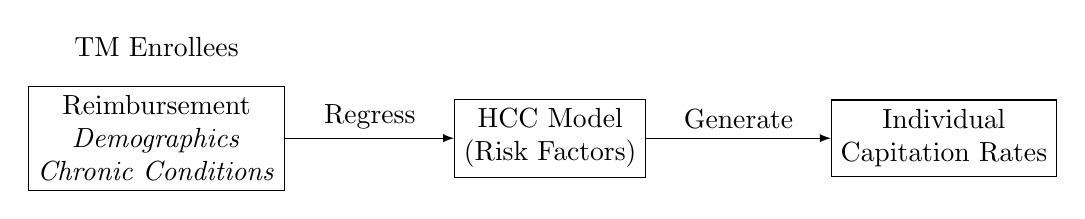
\begin{tikzpicture}
    \node[draw, rectangle, align=center] (input) at (0,0) { Reimbursement \\  \textit{Demographics}  \\  \textit{Chronic Conditions}};
    \node[above=0.25cm of input] {TM Enrollees};
    \node[draw, rectangle, align=center] (model) at (5,0) {HCC Model \\ (Risk Factors)};
    \node[draw, rectangle, align=center] (output) at (10,0) {Individual \\ Capitation Rates};
    
    \draw[->, >=latex] (input) -- (model) node[midway,above] {Regress};
    \draw[->, >=latex] (model) -- (output) node[midway,above] {Generate};
\end{tikzpicture}
    \caption{Capitation Rate Generation Process}
  \end{figure}
\end{frame}

\begin{frame}{Appendix: Risk Adjustment Outcomes}
  \begin{columns}
    \begin{column}{0.5\textwidth}
      \begin{figure}
        \centering
        \includegraphics[width=1\textwidth]{figures/images/avg_spending_vs_capitation_by_capitation_deciles.png}
        \caption{Conditional on Capitation Deciles}
      \end{figure}
    \end{column}
    \begin{column}{0.5\textwidth}
      \begin{figure}
        \centering
        \includegraphics[width=1\textwidth]{figures/images/avg_spending_vs_capitation_by_spending_deciles.png}
        \caption{Conditional on Spending Deciles}
      \end{figure}
    \end{column}
    
  \end{columns}
\end{frame}

\begin{frame}{Appendix: Benefit Structure}
  \begin{figure}
    \begin{figure}
      \centering
      \resizebox{0.8\textwidth}{!}{\usetikzlibrary{positioning, fit, backgrounds}
\begin{tikzpicture}[
    block/.style={
      draw,
      rectangle,
      rounded corners,
      minimum height=2cm, 
      minimum width=3cm, 
      align=center
    },
    node distance=0.5cm
]
% Nodes of MA coverage
\node[block] (ma) {Medicare Basic\\Part A\&B Coverage};
\node[block, right=of ma] (supp) {MA\\Supplementary\\Part A\&B Coverage};
% make the add node in dashed line
\node[block, right=of supp, dashed] (add) {Additional Benefits \\ (e.g. Dental)};

% group the nodes
\begin{scope}[on background layer]
    % add title MA Benefits over the nodes
  \node[above=0.5cm of supp] {Medicare Advantage};
  \node[fit=(ma) (supp) (add), draw, inner sep=0.5cm] (ma_group) {};
\end{scope}

% add space between the two groups
\node[below=1cm of ma_group] {};

% Nodes of Medigap coverage
\node[block, below=2cm of ma] (medigap) {Medicare Basic\\Part A\&B Coverage};
\node[block, right=of medigap] (medigap_supp) {Medigap\\Supplementary\\Part A\&B Coverage};


% group the nodes
\begin{scope}[on background layer]
    % add title Medigap Benefits over the nodes
  \node[above=0.5cm of medigap_supp] {TM+Medigap};
  \node[fit=(medigap) (medigap_supp), draw, inner sep=0.5cm] (medigap_group) {};
\end{scope}

\end{tikzpicture}}
    \end{figure}
  \end{figure}
\end{frame}

\end{document}